%%%%%
%%%%% File name  : hw3_report.tex
%%%%% Author     : Yueh-Chou Lee
%%%%% Date       : April 31, 2020
%%%%%
%%
%%%
\documentclass[a4paper,11pt]{article}
\usepackage[top=1.5cm,bottom=1.5cm,outer=2cm,inner=2cm]{geometry}
\usepackage[utf8]{inputenc}
\usepackage[T1]{fontenc}
\usepackage{fontspec}
\usepackage{xeCJK}
\usepackage{amsfonts}
\usepackage{amsmath}
\usepackage{graphicx}
\usepackage{subfigure}
\usepackage{setspace}
\usepackage[explicit]{titlesec}
\usepackage{titlesec}
\usepackage{bibentry}
\usepackage[nottoc,numbib]{tocbibind} 
\usepackage{filecontents}
\usepackage{color}
\renewcommand{\baselinestretch}{2}
\setCJKmainfont{標楷體}


\title{Machine Learning Homework 3 Report}
\author{R06221012\hspace{0.2cm}數學所\hspace{0.2cm}李岳洲}
\date{April 31, 2020}

\begin{document}

\maketitle

\begin{enumerate}
	\item \textit{\textbf{請說明你實作的 CNN 模型,其模型架構、訓練參數量和準確率為何?}}

	optimizer: Adam, learning rate: 0.0001, batchsize: 512, epoch: 300, early stopping patient: 30\\

		\begin{table}[htp]
			\begin{center}
				\begin{tabular}{ | c | c | c | c | c | c |}
				  	\hline
			  		& Training accuracy & Training loss & Validation accuracy & Validation loss & Test accuracy\\[0.5ex] 
			  		\hline \hline
			  		CNN & $0.971923$ & $0.000707$ & $0.829697$ & $0.001128$ & $0.85475$\\[0.2ex]
			  		\hline
				\end{tabular}
				\caption{CNN results}
			\end{center}
		\end{table}

		\begin{figure}[htp]
		    \begin{center}
		    		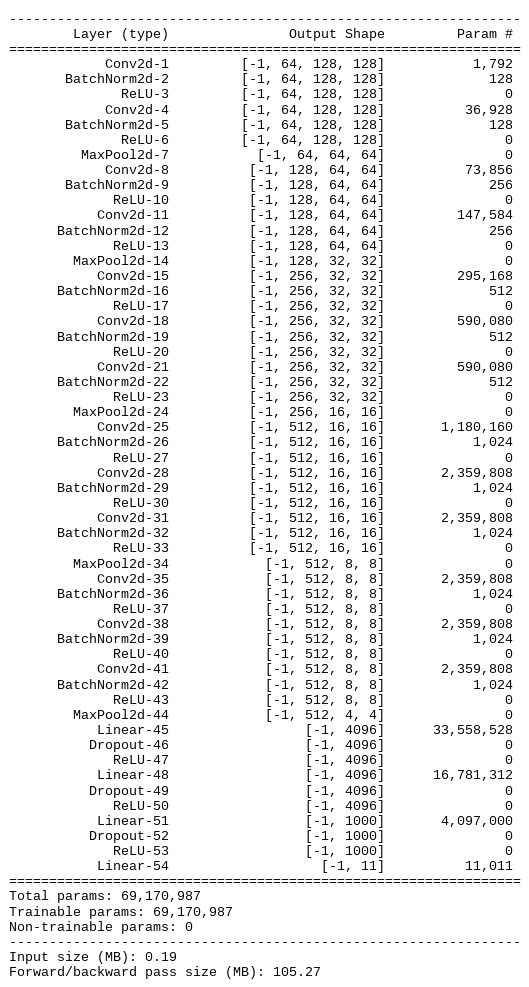
\includegraphics[scale=0.35]{./cnn_architecture.png}
		    	\caption{CNN model architecture}
		    \end{center}
		\end{figure}

\newpage

	\item \textit{\textbf{請實作與第一題接近的參數量,但 CNN 深度(CNN 層數)減半的模型,並說明其模型架構、訓練參數量和準確率為何?}}

	optimizer: Adam, learning rate: 0.0001, batchsize: 512, epoch: 300, early stopping patient: 30\\

		\begin{table}[htp]
			\begin{center}
				\begin{tabular}{ | c | c | c | c | c | c |}
				  	\hline
			  		& Training accuracy & Training loss & Validation accuracy & Validation loss & Test accuracy\\[0.5ex] 
			  		\hline \hline
			  		CNN (half layers) & $0.758362$ & $0.001420$ & $0.662767$ & $0.002215$ & --\\[0.2ex]
			  		\hline
				\end{tabular}
				\caption{CNN (half layers) results}
			\end{center}
		\end{table}

		\begin{figure}[htp]
		    \begin{center}
		    		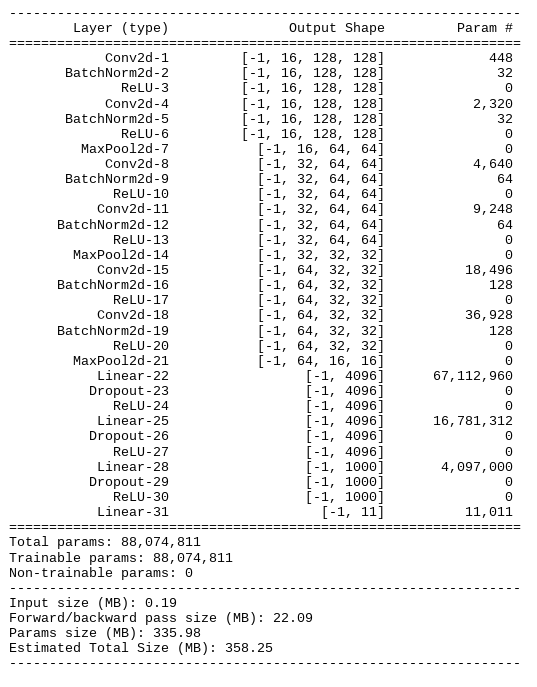
\includegraphics[scale=0.6]{./half_cnn_architecture.png}
		    	\caption{CNN model architecture (half layers)}
		    \end{center}
		\end{figure}

\newpage
	
	\item \textit{\textbf{請實作與第一題接近的參數量,簡單的 DNN 模型,同時也說明其模型架構、訓練參數和準確率為何?}}

	optimizer: Adam, learning rate: 0.0001, batchsize: 256, epoch: 300, early stopping patient: 30\\

		\begin{table}[htp]
			\begin{center}
				\begin{tabular}{ | c | c | c | c | c | c |}
				  	\hline
			  		& Training accuracy & Training loss & Validation accuracy & Validation loss & Test accuracy\\[0.5ex] 
			  		\hline \hline
			  		DNN & $0.417784$ & $0.006590$ & $0.390837$ & $0.007002$ & --\\[0.2ex]
			  		\hline
				\end{tabular}
				\caption{DNN results}
			\end{center}
		\end{table}

		\begin{figure}[htp]
		    \begin{center}
		    		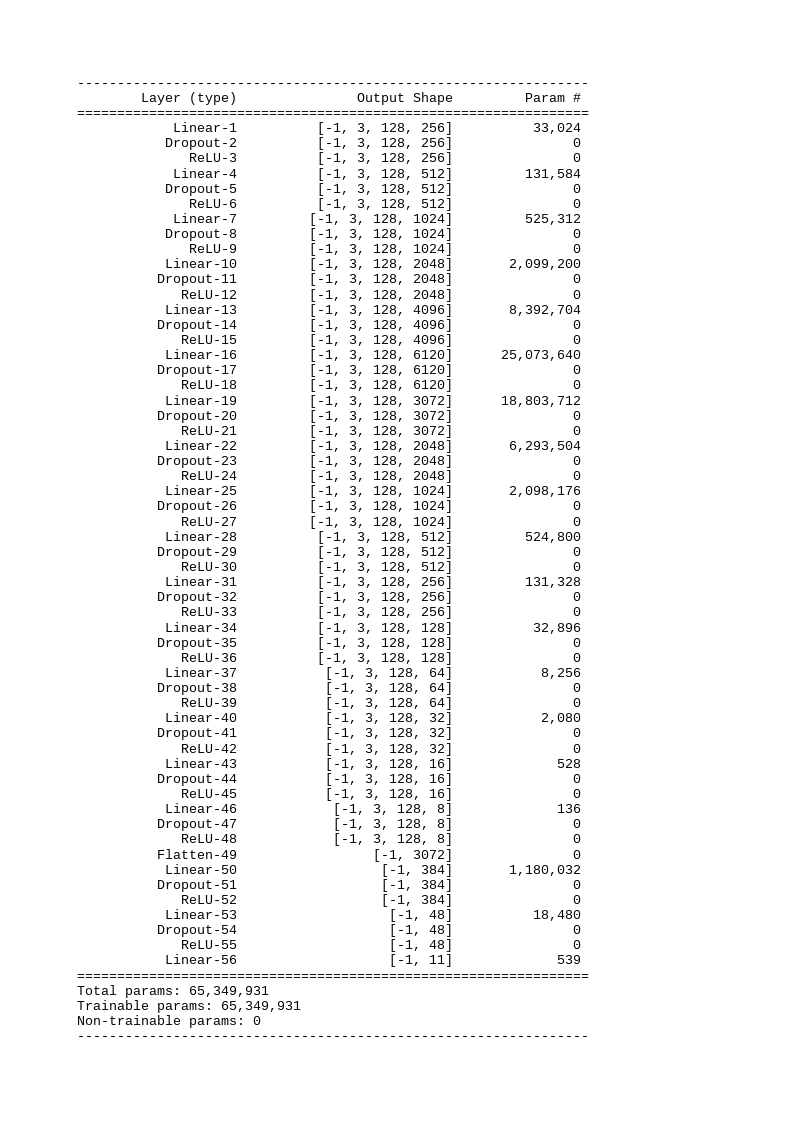
\includegraphics[scale=0.415]{./dnn_architecture.png}
		    	\caption{DNN model architecture}
		    \end{center}
		\end{figure}

\newpage

	\item \textit{\textbf{請說明由 1 $\sim$ 3 題的實驗中你觀察到了什麼?}}

	We use data normalization, data augmentation and early stopping in the above 1 $\sim$ 3. All of them are stopped before 300 epochs. 

	\item \textit{\textbf{請嘗試 data normalization 及 data augmentation,說明實作方法並且說明實行前後對準確率有什麼樣的影響?}}

	\begin{enumerate}
		\item Data normalizatin:

			Calculate the batch mean and standard deviation of training set, then apply this mean and standard deviation to validation set and testing set.

			\textbf{Usage:}

				\hspace{3cm} \textit{torchvision.transforms.Normalize(mean, std)}

		\item Data augmentation:

			Input size: $3 \times 128 \times 128$

			\begin{enumerate}
				\item[(i)] We resized to the size $3 \times 150 \times 150$, then randomly crop center by the size $3 \times 128 \times 128$.

				\item[(ii)] Randomly horizontal flip.

				\item[(iii)] Randomly rotation by degree $15$.

				\item[(iv)] Double the original dataset by augmentation.
			\end{enumerate}

			\textbf{Usage:}

				\hspace{3cm} (i) \textit{torchvision.transforms.Resize(150),}

    			\hspace{3.5cm}	\textit{torchvision.transforms.RandomResizedCrop(128)}

    			\hspace{3cm} (ii) \textit{torchvision.transforms.RandomHorizontalFlip()}

    			\hspace{3cm} (iii) \textit{transforms.RandomRotation(15)}

\newpage

		\item Comparison table:\\

			\begin{table}[htp]
				\begin{center}
					\begin{tabular}{ | c | c | c | c | c | c |}
					  	\hline
				  		& Training accuracy & Training loss & Validation accuracy & Validation loss & Test accuracy\\[0.5ex] 
				  		\hline \hline
				  		original cnn & $0.995231$ & $0.000439$ & $0.761623$ & -- & $0.78720$ \\[0.2ex]
				  		\hline
				  		augmentation & $0.928874$ & $0.000812$ & $0.776205$ & -- & $0.79438$ \\[0.2ex]
				  		\hline
				  		augmentation & & & & & \\
				  		+ & $0.971923$ & $0.000707$ & $0.829697$ & $0.001128$ & $0.85475$\\
				  		normalization & & & & & \\[0.2ex]
				  		\hline
					\end{tabular}
					\caption{Results comparison table}
				\end{center}
			\end{table}

	\end{enumerate}

	\item \textit{\textbf{觀察答錯的圖片中,哪些 class 彼此間容易用混?}}\\

		\begin{figure}[htp]
		    \begin{center}
		    		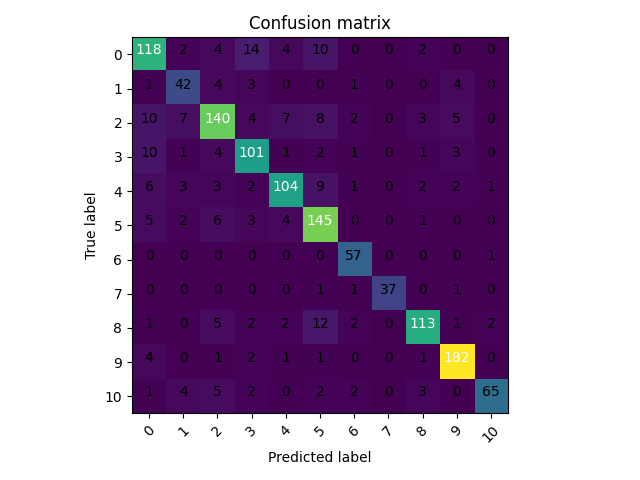
\includegraphics[scale=0.75]{./confusion_matrix.png}
		    	\caption{Confusion matrix}
		    \end{center}
		\end{figure}

		\begin{figure}[htp]
		    \begin{center}
		    	\subfigure[Class 0]{
		    		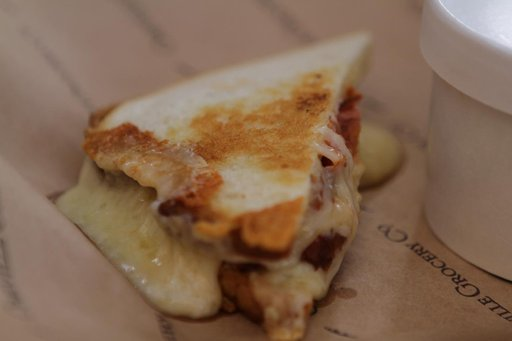
\includegraphics[height=2.5cm]{0.jpg}
		    	}
		    	\quad
		    	\subfigure[Class 2]{
		    		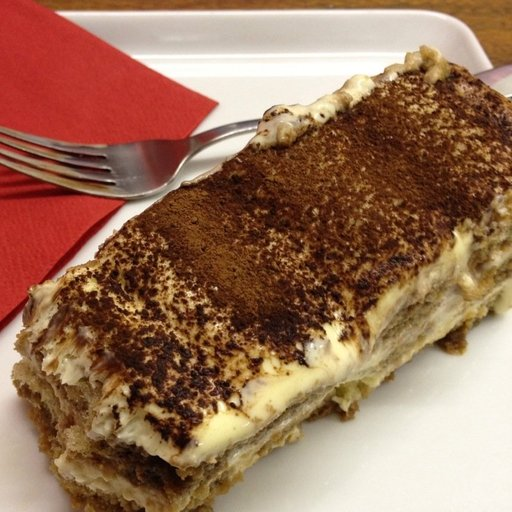
\includegraphics[height=2.5cm]{2.jpg}
		    	}
		    	\quad
		    	\subfigure[Class 3]{
		    		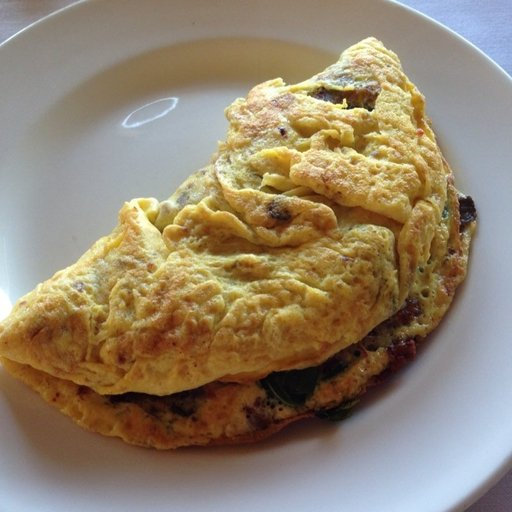
\includegraphics[height=2.5cm]{3.jpg}
		    	}
		    	\quad
		    	\subfigure[Class 5]{
		    		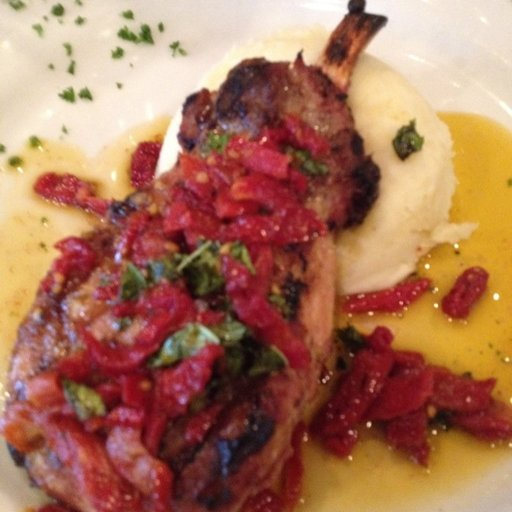
\includegraphics[height=2.5cm]{5.jpg}
		    	}
		    	\caption{Confused classes}
		    \end{center}
		\end{figure}
\end{enumerate}
\end{document}